\documentclass{article}
% main document, called main.tex
\usepackage{tikz}
\usetikzlibrary{external}

\usetikzlibrary{positioning}
\usetikzlibrary{calc}
\usetikzlibrary{shapes.geometric, arrows, arrows.meta}
\usepackage{varwidth}% http://ctan.org/pkg/varwidth
\usetikzlibrary{shadows,trees, mindmap}
\usetikzlibrary{matrix}
\usetikzlibrary{fit}

\tikzexternalize % activate!
\begin{document}
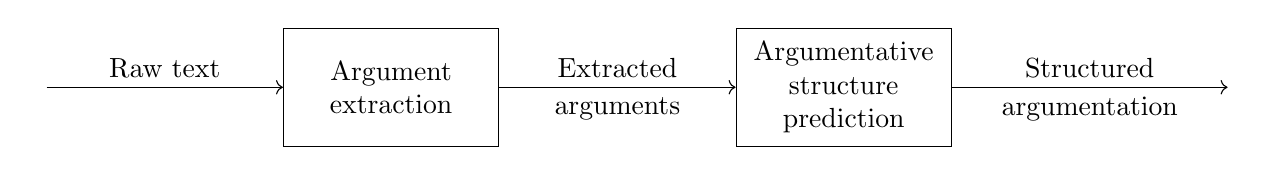
\begin{tikzpicture}
[box/.style={
rectangle, draw, text width=2.5cm, minimum height=1.5cm, align=center}
]
\node (most-left) {};
\node (argex) [box, right=3cm of most-left] {Argument extraction};
\node (argstruc) [box, right=3cm of argex] {Argumentative structure prediction}; 
\node (most-right) [right=3.5cm of argstruc] {};
\draw[->] (most-left) -- (argex) node [above, midway] {Raw text}; 
	\draw[->] (argstruc) -- (most-right) node [above, midway] {Structured} node [below, midway] {argumentation} ; 
	\draw[->] (argex) -- (argstruc) node [above, midway] {Extracted} node [below, midway] {arguments}; 
\end{tikzpicture}

\end{document}


